% Based on 
% http://www.texample.net/tikz/examples/red-black-tree/

\documentclass[12pt]{standalone}
\usepackage{tikz}
\usetikzlibrary{arrows}
\definecolor{color1}{RGB}{0,114,178}
\definecolor{color2}{RGB}{0,158,115}
\definecolor{color3}{RGB}{213,94,0}


\tikzset{
  treenode/.style = {align=center, inner sep=0pt, text centered,
    font=\sffamily},
  vertex/.style = {treenode, circle, black, font=\sffamily\bfseries, draw=color3,
    fill=color3, text width=0.3em},
}

\begin{document}
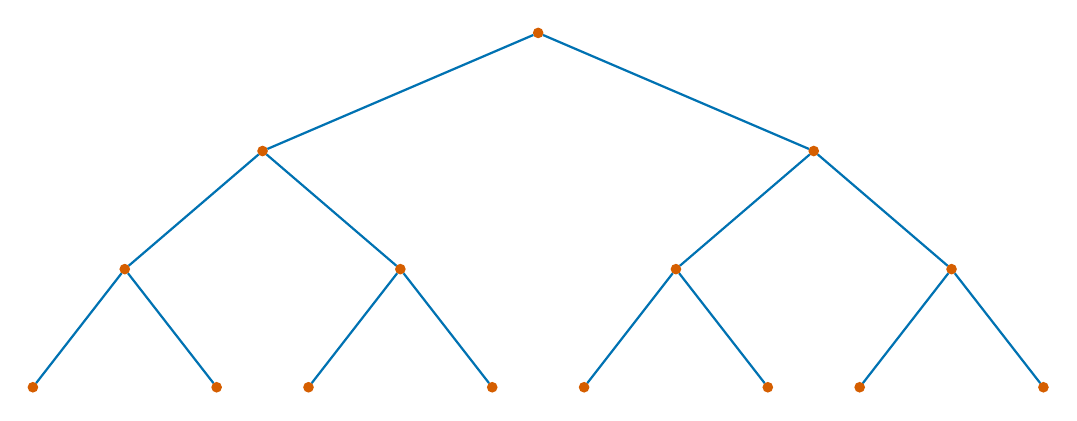
\begin{tikzpicture}[-,>=stealth',thick,draw=color1,level/.style={sibling distance = 7cm/#1,
  level distance = 1.5cm}] 
\node [vertex] {}
    child{ node [vertex] {} 
            child{ node [vertex] {} 
            	child{ node [vertex] {}            	
              }
            	child{ node [vertex] {}            	
              }
            }
            child{ node [vertex] {}
            	child{ node [vertex] {}            	
              }
            	child{ node [vertex] {}            	
              }
            }                            
    }
    child{ node [vertex] {}
            child{ node [vertex] {} 
							child{ node [vertex] {}}
							child{ node [vertex] {}}
            }
            child{ node [vertex] {}
							child{ node [vertex] {}}
							child{ node [vertex] {}}
            }
		}
; 
\end{tikzpicture}
\end{document}
